% !TeX root = ../main.tex
\chapter{实验内容}
\label{cha:chapter02}

\begin{figure}[H] % use float package if you want it here
  \centering
  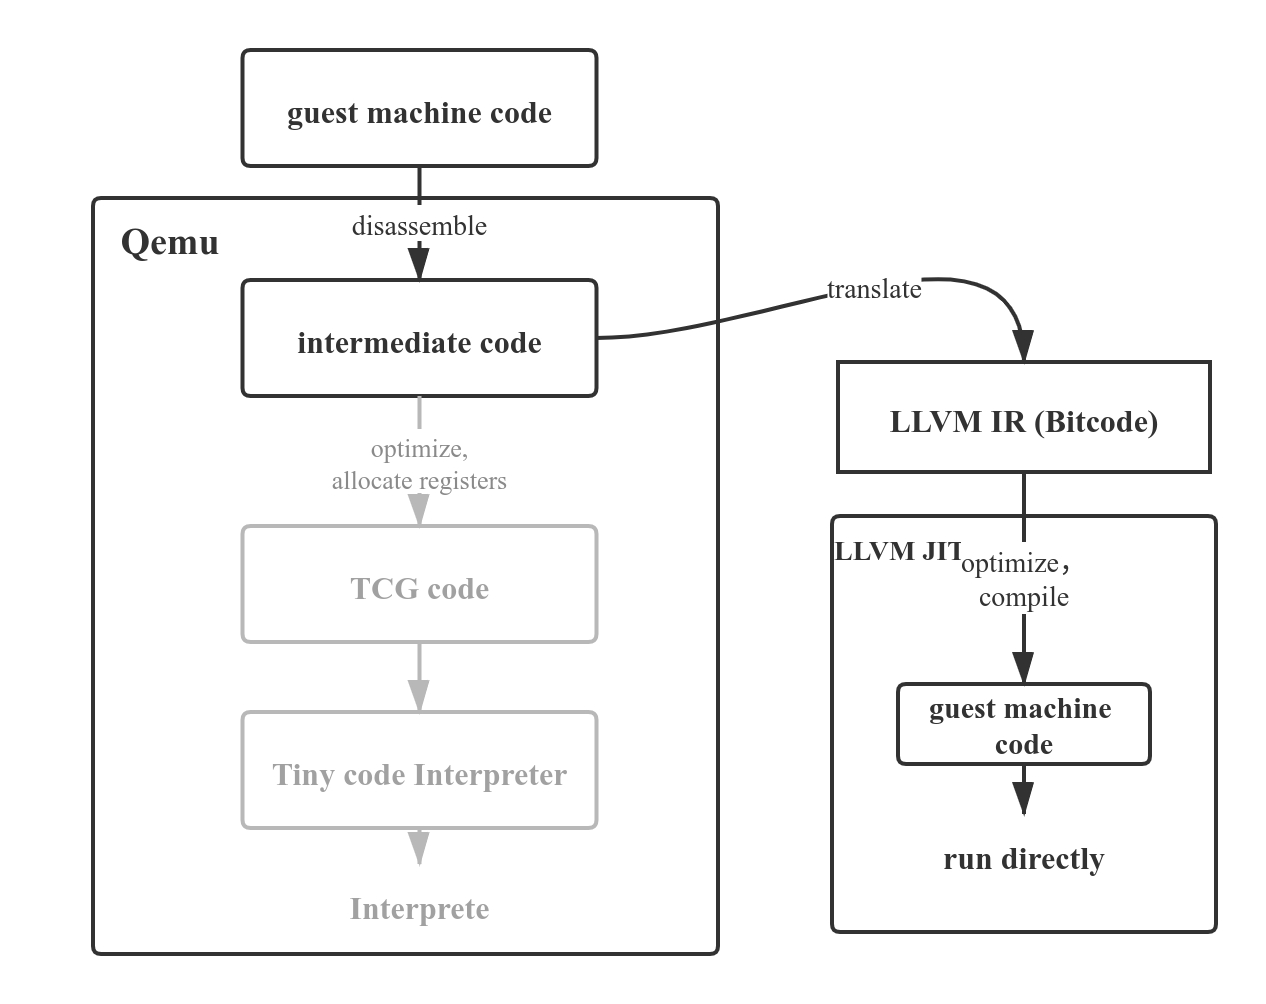
\includegraphics [width=0.80\textwidth]{p1.png}
  \caption{优化后的QEMU指令翻译,执行过程粗略图}
  \label{fig:xfig1}
\end{figure}

LLVM优化后的QEMU模拟器的指令翻译,执行过程如图2.1所示

\section{指令翻译得到LLVM IR}
    如图2.1所示, 在我的项目实现中,LLVM IR由客户程序的机器码反汇
    编得到的TCG中间代码翻译而得到。实际上LLVM IR也可以由机器码直
    接翻译得到, 但综合考虑代码实现的简便性, 代码的可读性, 以及后来的
    实验结果表明, 代码执行阶段带来的性能提升远远超过翻译时期的开销改变,
    于是采用了最终的实现方案, 即直接沿用了QEMU模拟器原有的反汇编过程。
    TCG中间代码包含了一系列TCG ops, 我手写代码完成了各类TCG ops向
    LLVM IR指令的转化工作。具体来说, 由机器码反汇编得到的TCG中间代码
    描述了一系列临时变量(最多达512个)之间的操作以及一些内存操作。我使用了
    一个包含512个LLVM临时变量的数组来存储执行时临时变量的值。内存操作
    通过使用一些辅助函数, 并绑定到相对应的LLVM函数来实现。这样, 每个TB
    的TCG中间代码, 都会逐条指令被翻译为LLVM指令, 并得到一个LLVM函数。
    当需要执行某个TB时, 就通过LLVM的执行引擎执行相对应的LLVM函数即可,
    TB对应的LLVM函数的返回值包含有最后执行到的TB所在地址以及跳转出口(0或1)。

\section{指令的执行}
    在翻译得到LLVM IR后, 就到了指令的执行阶段。LLVM对指令的执行提供了两种
    类型的执行引擎: JIT Compiler(即时编译器) 和 Interpreter(解释器)。
    JIT Compiler采用即时编译, 即在某个编译模块中的任意函数第一次被执行时,
    才编译整个模块, 进行IR优化并生成机器代码, 此后该编译模块中的函数被执行时,
    只需要执行相应的机器码即可; Interpreter则不编译生成机器码, 而是逐条指令
    解释执行LLVM IR, 也不负责进行任何IR优化。

    \begin{table}[htbp]
      \centering
      \caption{使用不同的执行引擎, 某一TB先后被执行多次的时间开销(us)}
      \label{tab:tabexamp1}
      \begin{minipage}[t]{0.9\textwidth}
        \begin{tabularx}{\linewidth}{|l|X|X|X|X|X|X|X|}
          \hline
          {\diagbox[width=7em]{执行引擎}{执行轮次}} & 1st & 2st & 3rd &4th &5th &6th &7th \\ \hline
          JIT Compiler& 7452.01 & 0.285& 0.294& 0.257 &0.227 &0.283 &0.207\\
          Interpreter& 70.748 & 66.999& 66.959& 67.504 & 66.727 &66.399 &66.828 \\
          regular qemu& 0.779 & 0.539& 0.491& 0.553 &0.430 &0.562 &0.490\\ \hline
        \end{tabularx}\\[2pt]
        \footnotesize \\
      \end{minipage}
    \end{table}

    表2.1是分别使用LLVM提供的JIT Compiler, Interpreter以及常规QEMU模拟器的TCI解释器
    作执行引擎, 执行某一测试程序时, 某一会被反复执行的特定TB在前7次被执行时的时间开销。通过表中数据可以
    得知, 在代码执行性能方面, LLVM提供的JIT Compiler在第一次执行时的编译过程会造成较大的延时,
    但由此带来的好处是后续执行用时的大幅度减少, 编译得到的机器码运行耗时约为常规QEMU使用TCI解释执行
    的50$\%$。而LLVM提供的Interpreter对IR解释执行的效率与常规QEMU模拟器相比, 仍有较大差距。至此, 我们可以
    确定, 使用LLVM提供的JIT编译器发射得到宿主机上的机器码, 相较于常规的QEMU模拟器, 可以通过牺牲第一次编译
    的时间成本, 换取执行时显著的性能提升。对于频繁执行的TB, 这样的牺牲是值得的, 这可以使QEMU模拟器的整体性能
    得到明显改善。

\section{性能评估}
    在项目实现过程中, 我尝试了多种不同的代码执行策略, 目的是尽可能提高QEMU模拟器的执行性能。为了定量地评估并比较
    各种实现策略下的QEMU模拟器的性能和相较常规QEMU模拟器的性能变化, 我使用NBench作为基准程序对优化后的QEMU进行测试。
    NBench(Native mode Benchmark)是一种合成计算基准程序, 开发于1990年代中期, 旨在测量计算机的CPU,FPU和
    内存系统速度。我使用改进后的qemu模拟器在用户态下执行另一平台架构的NBench程序, NBench程序会执行一系列计算任务,
    并给出CPU(qemu模拟器模拟的)的性能评分, 我将主要关注评测结果中的Integer Index指标。Integer Index是一系列
    仅涉及整数处理的的测试结果的几何平均值, 包括数字排序, 字符串排序, 位域操作, 模拟浮点, 任务分配, 霍夫曼编码, IDEA
    (国际数据加密算法)。该指数指出了被评测系统相较于90MHz奔腾Intel CPU的基准系统的相对性能分数,从而可以总体了解被
    测机器的性能。

\subsection{仅使用JIT Compiler作为执行引擎}
    起初, 我仅使用JIT Compiler作为QEMU的执行引擎, 即对于翻译得到的每一个TB,都在第一次执行时将LLVM IR编译为机器代码,
    然后执行这一段机器代码。这样的执行策略的缺点在于,对于那些执行频次较低的TB而言, 耗时的IR优化以及编译过程带来的执行期性能提升将
    是得不偿失的。LLVM提供的JIT Compiler可以被设置为四种不同的优化级别, 用数字0-3表示, 对应与即时编译时对IR的不同优化力度,
    优化级别为0, 表示不对IR执行任何优化, 3表示执行最高级别的优化。

    如表2.2所示, 我统计了仅使用LLVM JIT Compiler作为执行引擎, 并设置不同的优化级别时, 使用NBench测试所得到的Integer
    Index数值, 并与常规的QEMU模拟器进行了比较。由于此时我并未实现TB chaining机制, 出于性能比较的公平性, 在对比时我禁用了
    常规QEMU模拟器的TB chaining机制。

    \begin{table}[htbp]
    \begin{minipage}{0.8\textwidth}
    \centering
    \caption{使用JIT编译器作执行引擎, 并设置不同的代码优化级别得到的NBench评测结果}
    \label{tab:parallel1}
    \begin{tabular}{p{4cm}p{4cm}}
    \toprule[1.5pt]
    实现 & Integer Index \\\midrule[1pt]
    regular qemu, no tb chaining & 0.451 \\\midrule[1pt]
    llvm-qemu, opt-level = 0 & 0.971 \\\midrule[1pt]
    llvm-qemu, opt-level = 1 & 1.744 \\\midrule[1pt]
    llvm-qemu, opt-level = 2 & 1.756 \\\midrule[1pt]
    llvm-qemu, opt-level = 3 & 1.696 \\\bottomrule[1.5pt]
    \end{tabular}
    \end{minipage}%
    \end{table}

    从表中数据分析可知, 使用LLVM JIT Compiler作执行引擎, 即使不对IR执行任何优化(opt-level=0), 模拟CPU的性能也显著优于常规的
    QEMU模拟器, 在对LLVM IR进行一些优化(opt-level>0)后, 模拟CPU的性能进一步得到显著提升, 在优化级别为2时, 评测得到的Integer
    Index数值最高。当优化级别由2升高至3后, 性能评分反而略微降低。这一现象可以理解为过高的优化级别使得IR优化力度过大, 这带来的代码
    执行性能上的提升不足以弥补优化, 编译期的额外开销。实际上, JIT Compiler的默认优化级别为2, 将优化级别设置为3是更激进的做法, 并不是
    普适的选择。在实验的余下部分, 我都将JIT Compiler的优化级别设置为2(默认的优化级别)。

\subsection{将Interpreter与JIT Compiler结合使用}
    为了克服仅使用JIT Compiler作为执行引擎的缺点, 我实现了一种将Interpreter和JIT Compiler结合起来使用的简单的执行策略: 设置一个
    执行次数的阈值, 并为每一个TB设置一个被执行次数的计数器, 当需要执行一个TB时, 若该TB的被执行总次数未超过设定的阈值, 则使用LLVM提供的
    Interpreter直接逐指令地对该TB的LLVM IR解释执行,直到执行次数达到阈值时, 才使用JIT Compiler进行IR优化并生成机器码, 此后对该TB的执行
    都会直接运行机器码。我将执行频次达到阈值的TB称为热点(hotspot)TB, 这样的策略能优先对那些被认为会被多次执行的TB执行优化, 而对于那些执行频次低的
    TB, 执行期的性能提升不再那么重要, 使用Interpreter执行IR能避免编译带来的巨大开销。而根据著名的二八定律, 计算机在80$\%$的时间里执行20$\%$
    的常用代码, 这样的只对热点TB进行优化并编译的策略是具有较高的实际意义的。

    表2.2中展示了将执行频次阈值设置为5, 并对热点TB执行JIT编译, 非热点TB使用解释器解释执行, 带来的执行性能变化, 可见Integer Index相较于
    仅使用JIT编译时有略微提高。我使用的hotspot判定规则较为简单, 若结合实际执行情况使用更加复杂且合理的策略, 相信能得到更好的结果。

    \begin{table}[htbp]
    \begin{minipage}{0.8\textwidth}
    \centering
    \caption{对热点TB使用JIT编译, 非热点TB使用解释器解释执行, 得到的NBench评测结果}
    \label{tab:parallel1}
    \begin{tabular}{p{4cm}p{4cm}}
    \toprule[1.5pt]
    实现 & Integer Index \\\midrule[1pt]
    regular qemu, no tb chaining & 0.451 \\\midrule[1pt]
    llvm-qemu, opt-level = 2 & 1.756 \\\midrule[1pt]
    llvm-qemu, opt-level = 2, hotspot(threshold=5) & 1.804 \\\bottomrule[1.5pt]
    \end{tabular}
    \end{minipage}%
    \end{table}


\subsection{TB chaining的实现}
    由于在执行TB之前, 根据guest PC在多级缓存中查找对应TB地址的这一过程的性能开销可能较大, 所以我在我的项目实现中也使用了TB chaining机制,
    实现的原理与常规QEMU中的TB chaining相似, 区别之处在于, 常规QEMU在执行过程中需要记录下跳转的目的TB的TCG code的地址相对于上一TB的TCG code的相应跳转出口地址的偏移,
    在此后进行同一TB跳转时, 只需要在当前TCG code指针上加上这一偏移量, 就能接着执行下一个TB的TCG code; 而由于LLVM IR在优化并编译为机器码后, 将难以定位LLVM IR中的特定指令,
    这使得在TB对应的机器码之间执行跳转是不现实的, 而且在机器码层次执行跳转, 将会违背将TB作为执行单元的原则, 难以将每一TB作为独立个体分别执行优化力度的控制等,于是我的方案是对于每一个TB, 在执行过程中记录下
    每个跳转出口跳转至的TB的地址(即将TB链接起来), 在执行TB时, 将顺着这一链接关系一路执行下去, 直到无法通过链接关系定位下一TB为止。

    表2.3比较了使用LLVM优化的qemu模拟器在实现TB chaining前后的Nbench评测结果。可以看到性能显著提升, Integer Index相较未实现TB chaining时提升了68.7$\%$。


    \begin{table}[htbp]
    \begin{minipage}{0.8\textwidth}
    \centering
    \caption{实现TB chaining机制后, 得到的NBench评测结果}
    \label{tab:parallel1}
    \begin{tabular}{p{4cm}p{4cm}}
    \toprule[1.5pt]
    实现 & Integer Index \\\midrule[1pt]
    regular qemu, tb chaining implemented & 0.542 \\\midrule[1pt]
    llvm-qemu, opt-level = 2, hotspot(threshold=5), no TB chaining implemented & 1.804 \\\midrule[1pt]
    llvm-qemu, opt-level = 2, hotspot(threshold=5), TB chaining implemented & 3.044 \\\bottomrule[1.5pt]
    \end{tabular}
    \end{minipage}%
    \end{table}

    在进行了上述的优化和改进后, 最终得到的项目, 相较于常规的QEMU模拟器, 在64位ARM架构上运行x86程序的性能得到了大幅度提升, NBench
    下的评测结果显示, Integer Index增长为原来的5.62倍。

\section{实验总结}
    我认为该项目的实现有着重要的实际意义, 由于LLVM在代码优化上的强大能力以及它能根据特定的机器架构执行优化这一特点, 使用LLVM改善QEMU模拟器的指令翻译机制, 对于模拟器的性能提升是有很大潜力。
    我的实验证实了使用LLVM提供的工具链改善QEMU性能的可行性, 并为优化后的性能提升提供了数据支持, 对今后可能开展的使用LLVM对QEMU模拟器进行优化的工作有一定的借鉴意义。通过牺牲一定的编译时性
    能开销, 换取执行时性能的大幅度提升, 这使得x86真实应用在ARM架构机器上的可用性得到提升。目前还存在一些值得展开的后续工作: 首先, 由于本人的能力和时间有限, 目前仅实现了QEMU用户态下的优化工作,
    全系统模拟尚未实现成功, 将优化工作扩展到全系统态, 将使得在ARM架构上完全模拟x86时的性能得到明显提升; 我在对LLVM IR进行优化并编译生成机器码时, 采用了统一的优化级别, 更加合理的做法应该是
    根据TB的具体执行情况(被执行次数等), 动态地调节对IR的优化力度, 这样能更充分合理地挖掘优化带来的性能提升潜力; 同时, 对热点TB的判定可以采用更加复杂, 合理的策略, 而不是简单地依据TB的总被执行次数。
    这些都有待于在后续工作中加以改进完善。


